% !TEX root = ../main.tex

\section{Introduction and Paper Summary}

Retention time (RT) prediction is a core problem in LC-MS analysis because RT provides information that is complementary to MS/MS spectra. In the target paper, Kang et al.\ proposed \textbf{DeepGCN-RT}, a deep graph neural network for small-molecule RT prediction, and argued that previous RT-GNN models were still relatively shallow. Their main claim is that a \textbf{16-layer} graph convolutional architecture can be trained effectively once \textbf{residual connections}, \textbf{edge-aware message passing}, and an \textbf{attention/GRU readout} are introduced \cite{kang2023deepgcnrt}.

The paper reports three main contributions. First, on the SMRT benchmark, DeepGCN-RT improves the previously reported state of the art and reaches a test MAE of \textbf{26.55 s} and a MAPE of \textbf{0.033} (3.3\%). Second, after transfer learning from SMRT, the model improves performance on seven external chromatographic datasets with different conditions. Third, the authors show that predicted RT can help molecular identification on the RIKEN-PlaSMA dataset by filtering candidate structures before final ranking.

Our project focuses on an \textbf{independent PyTorch Geometric reimplementation} of the paper's core model and training pipeline. We used the authors' official repository only to clarify underspecified choices such as the readout structure, output normalization, and the exact transfer-learning hyperparameters. The final code in this repository was written independently and integrated into a clean training pipeline centered on PyG datasets, PyG data loaders, and our own \path{Networks/DeepGCNRT.py}. In the current report, we analyze three settings separately: SMRT base-model training, a separate SMRT\(\rightarrow\)RIKENMONA refinement experiment, and direct SMRT-initialized transfer learning on each MiniDataset under \textbf{10-fold evaluation}. This separation lets us keep the MiniDataset comparison closer to the paper's direct-transfer protocol while still reporting the intermediate RIKENMONA behavior.

\section{Model Architecture Reimplementation}

\subsection{Graph Construction}

Each molecule is converted from a canonical SMILES string into a graph
\(
G = (V, E)
\),
where atoms are nodes and bonds are directed edges. The preprocessing and featurization code in this repository produces node features of dimension \textbf{164} and edge features of dimension \textbf{11}. This closely follows the feature design described in the paper and the earlier GCN work by Kensert et al., which the paper explicitly adopts \cite{kang2023deepgcnrt}.

The node representation contains 20 groups of atom-level features, including element type, degree, formal charge, hybridization, aromaticity, hydrogen-bond donor/acceptor flags, ring membership, chirality-related features, and several RDKit-derived physicochemical contributions. Edge features contain 5 groups of bond-level attributes, including bond type, stereo information, conjugation, ring membership, and rotatability.

\subsection{Message Passing Layer}

The reimplemented model follows the paper's notation as closely as possible. Let
\(
\mathbf{h}^{(l)}_u \in \mathbb{R}^d
\)
denote the hidden representation of source node \(u\) at layer \(l\), and let
\(
\mathbf{h}^{(l)}_{e_{uv}} \in \mathbb{R}^d
\)
denote the encoded edge feature between \(u\) and \(v\). The edge-aware message is

\begin{equation}
\mathbf{m}^{(l)}_{uv} = \mathbf{h}^{(l)}_u + \mathbf{h}^{(l)}_{e_{uv}} .
\end{equation}

Following the best-performing setting used by the authors' released code, our implementation uses the \texttt{no\_relu} aggregation variant, so the attention weight is computed directly from the message:

\begin{equation}
\alpha^{(l)}_{uv} =
\frac{\exp \left( \mathbf{m}^{(l)}_{uv} \right)}
{\sum\limits_{u' \in \mathcal{N}(v)} \exp \left( \mathbf{m}^{(l)}_{u'v} \right)} .
\end{equation}

Messages are aggregated at the destination node by weighted summation:

\begin{equation}
\mathbf{m}^{(l)}_v =
\sum\limits_{u \in \mathcal{N}(v)}
\alpha^{(l)}_{uv} \odot \mathbf{m}^{(l)}_{uv} .
\end{equation}

The node state is then updated by a linear layer, ReLU, dropout, and residual connection:

\begin{equation}
\mathbf{h}^{(l+1)}_v =
\mathrm{Norm}
\left(
\mathrm{Dropout}
\left(
\mathrm{ReLU}
\left(
W^{(l)} \mathbf{m}^{(l)}_v
\right)
\right)
\;+\;
\mathbf{h}^{(l)}_v
\right).
\end{equation}

In our final configuration, \(\mathrm{Norm}\) is the identity map, which matches the released DeepGCN-RT implementation for the edge-aware residual model.

\subsection{Readout and Prediction Head}

After \(L=16\) graph convolution layers, molecule-level embeddings are produced by an attentive readout with two refinement steps. The initial graph state is the sum of node embeddings:

\begin{equation}
\mathbf{g}^{(0)} = \sum_{v \in V} \mathbf{h}^{(L)}_v .
\end{equation}

At each readout step, a graph-attention module propagates information from nodes to the graph state, and a GRU cell updates the graph embedding:

\begin{equation}
\mathbf{c}^{(k)} = \mathrm{GAT}\!\left(\{\mathbf{h}^{(L)}_v\}, \mathbf{g}^{(k-1)}\right),
\qquad
\mathbf{g}^{(k)} = \mathrm{GRU}\!\left(\mathbf{c}^{(k)}, \mathbf{g}^{(k-1)}\right).
\end{equation}

The final molecular representation is passed through a two-layer MLP:
\[
\mathbb{R}^{200} \rightarrow \mathbb{R}^{1024} \rightarrow \mathbb{R}^{1},
\]
with a ReLU between the two linear layers. The scalar output is the predicted RT in seconds.

\begin{algorithm}[t]
\caption{Forward Pass of Our DeepGCN-RT Reimplementation}
\begin{algorithmic}[1]
\State Encode atom features with a linear layer: \(\mathbf{x}_v \mapsto \mathbf{h}^{(0)}_v\)
\State Encode bond features with a linear layer: \(\mathbf{e}_{uv} \mapsto \mathbf{h}^{(0)}_{e_{uv}}\)
\For{\(l = 0, \dots, 15\)}
    \State Compute edge-aware messages \(\mathbf{m}^{(l)}_{uv}\)
    \State Aggregate incoming messages with softmax-normalized weights
    \State Apply linear layer, ReLU, dropout, and residual connection
\EndFor
\State Initialize graph embedding by sum pooling over all nodes
\For{\(k = 1, 2\)}
    \State Update graph embedding with graph attention and a GRU cell
\EndFor
\State Predict RT with the MLP head
\end{algorithmic}
\end{algorithm}

\subsection{Assumptions and Design Decisions}

Several details are not fully specified in the paper text, so we made the following explicit choices:

\begin{enumerate}
    \item \textbf{Independent framework choice.} The authors' code is written with DGL. We reimplemented the same layer structure in \textbf{PyTorch Geometric}, using \texttt{GATConv}, \texttt{global\_add\_pool}, and \texttt{GRUCell}. This changes the framework, but not the intended computation graph.
    \item \textbf{Output normalization.} The released DeepGCN-RT code uses \texttt{output\_norm="none"} for the edge-aware attentive model. We follow that setting.
    \item \textbf{Aggregation update function.} The released code exposes three options: \path{relu_eps_beta}, \path{relu}, and \path{no_relu}. We adopt \path{no_relu}, because it is the default path used by the published training scripts for DeepGCN-RT.
    \item \textbf{Readout initialization.} The paper states that the initial graph embedding is obtained by summing node embeddings before the GRU refinement. Our readout reproduces exactly that behavior.
    \item \textbf{Loss implementation.} The paper reports Huber loss. In PyTorch, \texttt{SmoothL1Loss} is the standard Huber-style implementation, so we use it as the training objective.
\end{enumerate}

\section{Implementation Details}

The codebase was reorganized around three layers:

\begin{enumerate}
    \item \textbf{Dataset modules.} \path{Datasets/SMRT.py}, \path{Datasets/MiniDatasets.py}, and \path{Datasets/RIKENMONA.py} expose a shared interface for preparing raw data, building PyG graphs, and loading train/validation/test splits.
    \item \textbf{Model definition.} \path{Networks/DeepGCNRT.py} contains the atom encoder, bond encoder, 16 residual edge-aware GCN layers, attentive readout, and final prediction head.
    \item \textbf{Training utilities.} \path{Train/lib/train_graph.py} implements the epoch loop, early stopping, scheduler stepping, checkpoint selection by validation loss, and metric logging.
\end{enumerate}

The implementation keeps the paper's layer widths and high-level structure unchanged: hidden dimension \(d=200\), 16 message-passing layers, two attentive readout steps, a 1024-unit dense hidden layer, dropout \(=0.1\), Adam optimizer, cosine warm restarts, and early stopping with patience 30.

One practical difference from the original repository is that our code unifies pretraining, transfer learning, and extra evaluation under the same training interface. This makes the pipeline easier to read and reuse. In the current version, we reproduce the \textbf{10-fold} transfer-learning loop, but we have \emph{not} yet repeated it for 10 different seeds, and we have not reimplemented the MSFinder-assisted candidate-filtering workflow used in the paper's RIKEN study.

\section{Experimental Setup}

\subsection{Datasets and Preprocessing}

We used all datasets prepared in the repository. Table~\ref{tab:datasets} summarizes their sizes and the split sizes actually used by our current code.

\begin{table}[t]
\centering
\caption{Datasets used in this project and the split sizes produced by our current loader (\(80\%/10\%/10\%\) after shuffling). All RT values are stored in seconds.}
\label{tab:datasets}
\resizebox{\textwidth}{!}{
\begin{tabular}{lrrrrl}
\toprule
Dataset & Total & Train & Valid & Test & Role in Report \\
\midrule
SMRT & 77,980 & 62,384 & 7,798 & 7,798 & Base pretraining dataset \\
RIKENMONA & 434 & 347 & 43 & 44 & Intermediate transfer / refinement stage \\
Cao\_HILIC\_116 & 116 & 92 & 12 & 12 & Downstream MiniDataset evaluation \\
Eawag\_XBridgeC18\_364 & 364 & 291 & 36 & 37 & Downstream MiniDataset evaluation \\
FEM\_lipids\_72 & 72 & 57 & 7 & 8 & Downstream MiniDataset evaluation \\
FEM\_long\_412 & 412 & 329 & 41 & 42 & Downstream MiniDataset evaluation \\
FEM\_short\_73 & 73 & 58 & 7 & 8 & Downstream MiniDataset evaluation \\
IPB\_Halle\_82 & 82 & 65 & 8 & 9 & Downstream MiniDataset evaluation \\
LIFE\_new\_184 & 184 & 147 & 18 & 19 & Downstream MiniDataset evaluation \\
LIFE\_old\_194 & 194 & 155 & 19 & 20 & Downstream MiniDataset evaluation \\
MTBLS87\_147 & 147 & 117 & 15 & 15 & Downstream MiniDataset evaluation \\
UniToyama\_Atlantis\_143 & 143 & 114 & 14 & 15 & Downstream MiniDataset evaluation \\
\bottomrule
\end{tabular}
}
\end{table}

The preprocessing pipeline is identical across datasets:

\begin{enumerate}
    \item remove empty export columns such as \path{Unnamed:*};
    \item drop rows with missing RT or unparsable molecular structure;
    \item prefer SMILES, fall back to InChI when needed;
    \item canonicalize molecules with RDKit;
    \item convert RT to seconds;
    \item transform molecules into PyG graphs and cache them to disk.
\end{enumerate}

One dataset-specific adjustment is important: in the MiniDatasets collection, the raw Excel files store RT in \textbf{minutes}, so our preprocessing multiplies those values by \(60.0\) before training. SMRT and RIKENMONA are already kept on the paper's second-based scale.

\subsection{Training Configuration}

Table~\ref{tab:training} lists the hyperparameters used in the code that generated the results currently stored in \path{Train/Results/DeepGCNRT/}.

\begin{table}[t]
\centering
\caption{Training settings used for the runs discussed in this report. The MiniDataset comparison uses the direct SMRT-initialized 10-fold runs stored under \texttt{Train/Results/DeepGCNRT/MiniDatasets/}.}
\label{tab:training}
\resizebox{\textwidth}{!}{
\begin{tabular}{llllll}
\toprule
Stage & Target dataset(s) & Initialization & Batch size & Epoch cap & Notes \\
\midrule
Stage 1 & SMRT & Random initialization & 64 & 200 & Base model training \\
Stage 2 & RIKENMONA & Best SMRT checkpoint & 64 & 200 & Separate refinement / analysis run \\
Stage 3 & Each MiniDataset & Best SMRT checkpoint & 64 & 200 & Direct transfer with 10-fold evaluation \\
\bottomrule
\end{tabular}
}
\end{table}

The following hyperparameters are shared across all three stages unless otherwise noted: 16 GCN layers, hidden dimension 200, two attentive readout steps, prediction head \(200 \rightarrow 1024 \rightarrow 1\), dropout 0.1, Adam optimizer, \texttt{CosineAnnealingWarmRestarts} with \(T_0 = 200\), \texttt{SmoothL1Loss}, early stopping patience 30, and random seed 42.

\subsection{Deviations from the Original Experimental Protocol}

Reproduction reports are only useful when deviations are stated clearly. The most important differences between our current implementation and the paper are listed in Table~\ref{tab:deviations}.

\begin{table}[t]
\centering
\caption{Explicit deviations from the original paper and why they matter.}
\label{tab:deviations}
\resizebox{\textwidth}{!}{
\begin{tabular}{p{3.2cm}p{5.1cm}p{5.1cm}p{4.1cm}}
\toprule
Aspect & Paper / official protocol & Our current implementation & Expected impact \\
\midrule
SMRT split & Fixed official split: 70,182 train and 7,798 test; train further split 9:1 for validation & \path{SMRT_train_set.txt} and \path{SMRT_test_set.txt} are merged, then reshuffled into 62,384/7,798/7,798 & Makes SMRT results \emph{not strictly directly comparable} to the paper's reported test score \\
Transfer evaluation & 10 rounds of 10-fold cross-validation, averaged over seeds; batch size 8 & One seed with 10-fold evaluation; batch size 64 & Matches the fold-wise averaging rule, but still uses fewer repetitions and different optimization dynamics \\
Checkpoint selection & Official transfer script selects the best checkpoint using the held-out fold itself & Our code keeps a separate validation split inside the training portion of each fold & Cleaner evaluation, but usually less optimistic than the official script \\
Transfer dataset scope & Paper discusses 7 external RPLC datasets & We also ran Cao\_HILIC\_116, FEM\_short\_73, and MTBLS87\_147 because they appear in the released codebase & Extra coverage, but those rows are supplementary rather than main-paper reproduction \\
RIKEN experiment & MSFinder-assisted candidate filtering and top-\(k\) identification accuracy & Current repo reproduces only the RT-regression refinement stage on RIKENMONA & We reproduce only part of the full identification workflow \\
Repetition strategy & 3 runs on SMRT; 10\(\times\)10 CV on transfer learning & One SMRT run, one RIKEN run, and one 10-fold transfer run per MiniDataset & Transfer variance is reduced relative to a single split, but still lacks the paper's multi-seed averaging \\
\bottomrule
\end{tabular}
}
\end{table}

\section{Results and Comparison}

\subsection{SMRT Benchmark}

Table~\ref{tab:smrt-main} compares our SMRT result against the values reported in the paper. Our reimplementation reaches a test MAE of \textbf{26.65 s}, which is numerically very close to the published \textbf{26.55 s}. The MedAE and MAPE are also close.

\begin{table}[t]
\centering
\caption{SMRT test-set performance. Baseline values are reproduced from Table 1 of the paper \cite{kang2023deepgcnrt}.}
\label{tab:smrt-main}
\begin{tabular}{lcccc}
\toprule
Method & MAE (s) & MedAE (s) & MAPE & \(R^2\) \\
\midrule
DeepGCN-RT (paper) & 26.55 & 12.38 & 0.033 & 0.89 \\
DeepGCN-RT (ours) & 26.65 & 12.53 & 0.033 & 0.90 \\
GCN (paper) & 29.40 & 15.02 & 0.040 & 0.89 \\
DNNpwa (paper) & 39.62 & 25.08 & 0.050 & 0.85 \\
GNN-RT (paper) & 39.87 & 25.24 & 0.050 & 0.85 \\
\bottomrule
\end{tabular}
\end{table}

At the best validation epoch (\(176\)), our SMRT run achieved validation/test MAE values of \(27.13/26.65\) s and validation/test \(R^2\) values of \(0.880/0.900\). This is strong evidence that the \textbf{architecture itself} has been reimplemented correctly.

However, this table should be interpreted cautiously. Our SMRT split is \emph{not} the same as the paper's split. Because we merged the published train and test files before reshuffling, our test set differs from the official held-out test set used by Kang et al. Therefore, the close match is encouraging, but not a strict apples-to-apples reproduction.

\begin{figure}[t]
\centering
\IfFileExists{Figures/smrt_base_scatter_report.png}{
    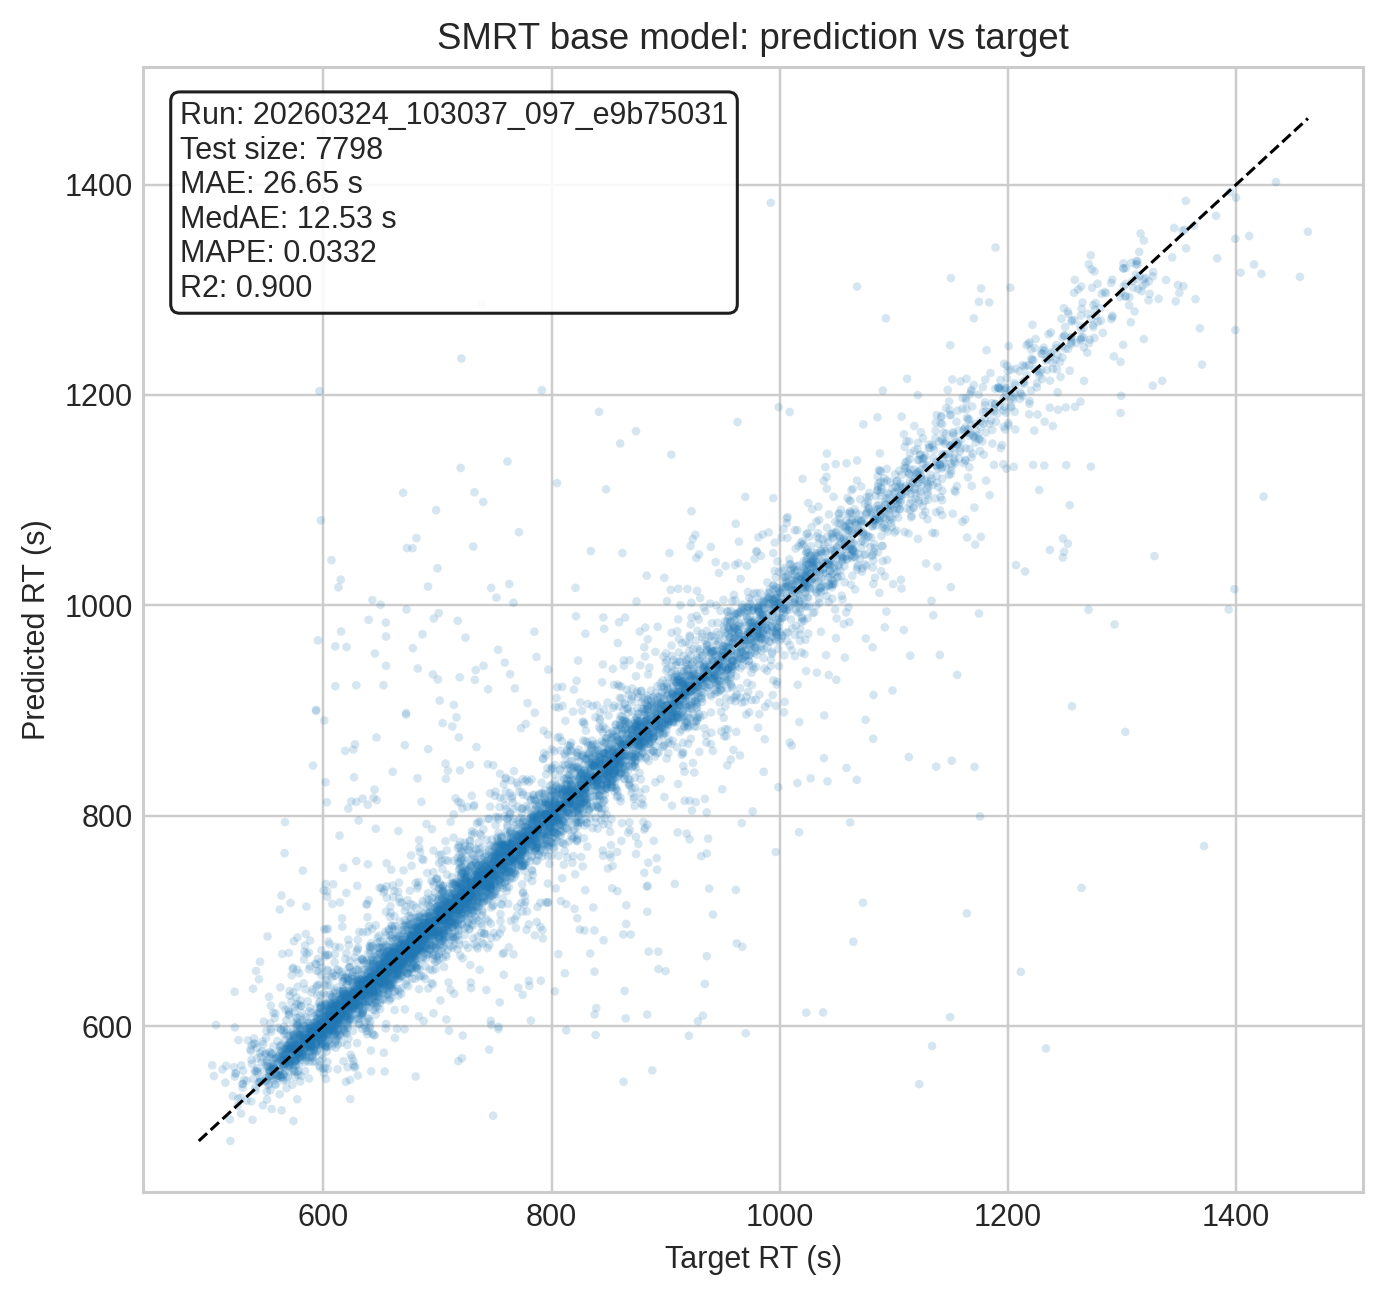
\includegraphics[width=0.72\textwidth]{Figures/smrt_base_scatter_report.png}
}{
    \fbox{\parbox{0.8\textwidth}{Run \texttt{Report/Figures/Figures.ipynb} to generate \texttt{smrt\_base\_scatter\_report.png}.}}
}
\caption{Prediction scatter plot for the SMRT base model. The notebook code saves this figure to \texttt{Report/Figures/smrt\_base\_scatter\_report.png}.}
\label{fig:smrt-scatter}
\end{figure}

\begin{figure}[t]
\centering
\IfFileExists{Figures/smrt_mae_comparison_report.png}{
    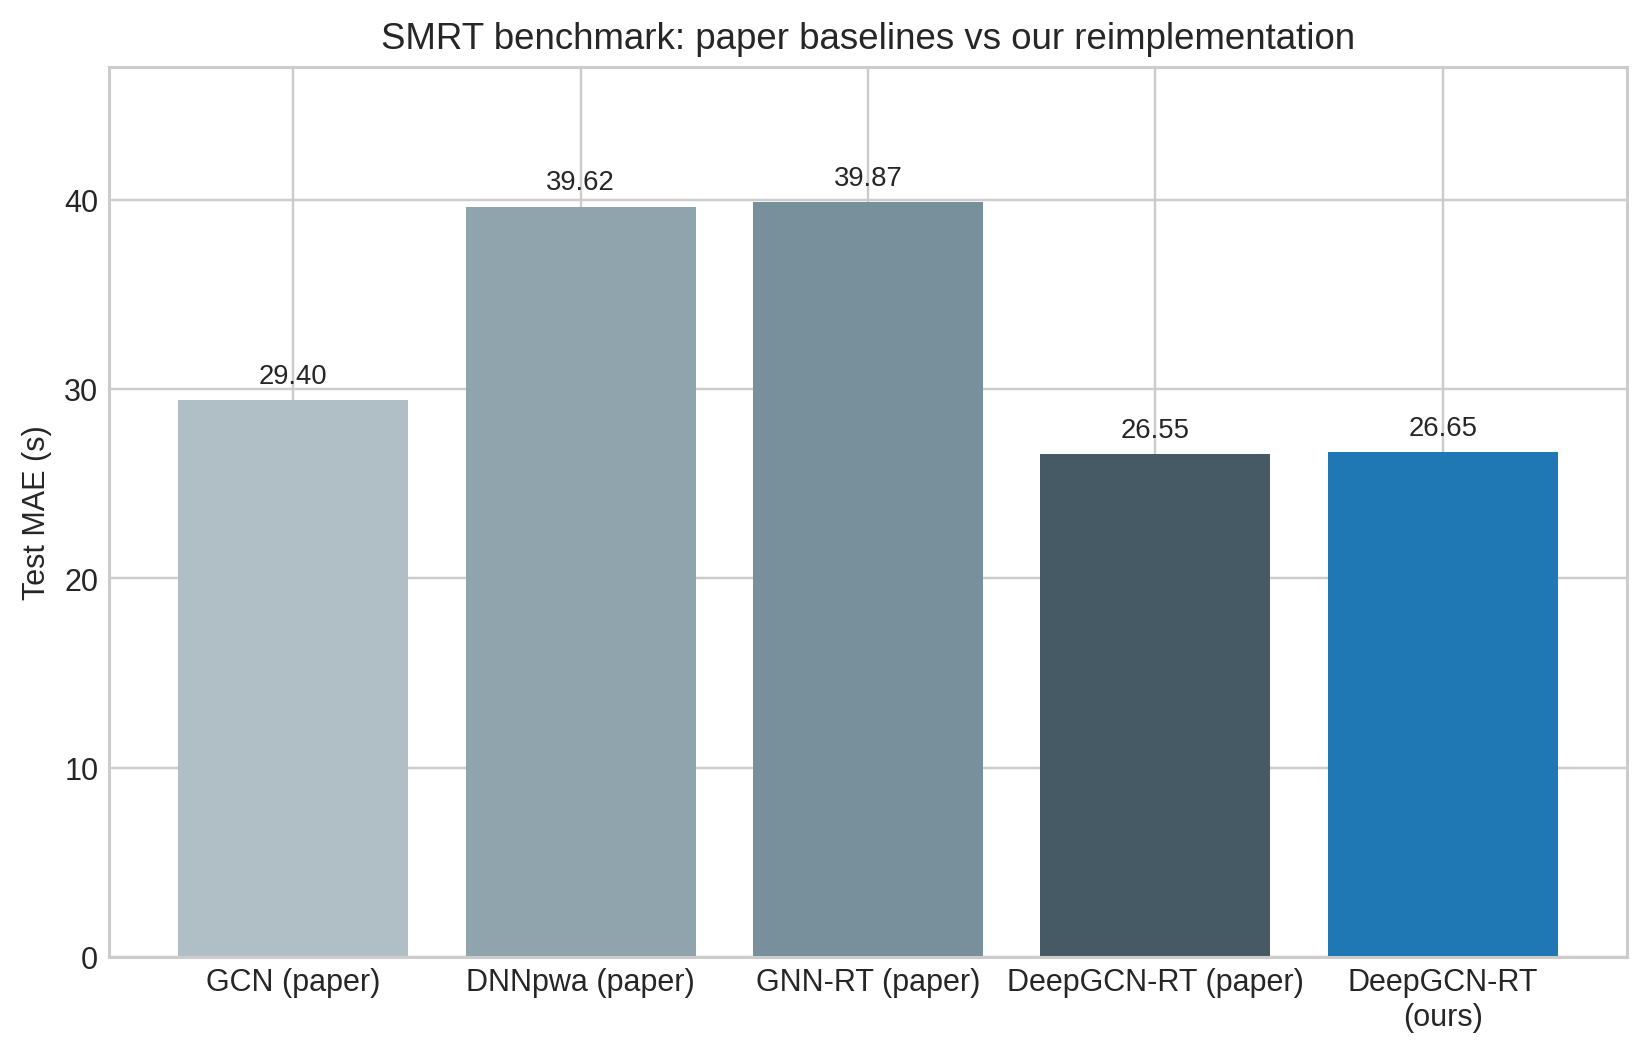
\includegraphics[width=0.74\textwidth]{Figures/smrt_mae_comparison_report.png}
}{
    \fbox{\parbox{0.8\textwidth}{Run \texttt{Report/Figures/Figures.ipynb} to generate \texttt{smrt\_mae\_comparison\_report.png}.}}
}
\caption{SMRT test MAE comparison between the paper's baselines and our reimplementation. Our MAE remains very close to the paper's DeepGCN-RT value and clearly below the earlier baselines reported in the paper.}
\label{fig:smrt-mae}
\end{figure}

\subsection{RIKENMONA Refinement Stage}

Separately from the paper-style MiniDataset benchmark, we fine-tuned the SMRT checkpoint on RIKENMONA to inspect whether the base representation transfers to a much smaller RT dataset. Table~\ref{tab:riken} reports the RT-regression performance of this refinement stage.

\begin{table}[t]
\centering
\caption{RIKENMONA refinement result using the SMRT-pretrained checkpoint.}
\label{tab:riken}
\begin{tabular}{lcccc}
\toprule
Setting & MAE (s) & MedAE (s) & MAPE & \(R^2\) \\
\midrule
RIKENMONA transfer model (ours) & 23.38 & 18.26 & 0.0892 & 0.828 \\
\bottomrule
\end{tabular}
\end{table}

This result is useful in two ways. First, it shows that the SMRT-pretrained representation transfers meaningfully to a much smaller RT dataset. Second, it gives us a concrete reference point for the part of the paper that later feeds into molecular identification. However, this should \emph{not} be described as a reproduction of the paper's full RIKEN-PlaSMA experiment, because the top-\(k\) MSFinder-assisted ranking stage was not reproduced.

\begin{figure}[t]
\centering
\IfFileExists{Figures/riken_refined_scatter_report.png}{
    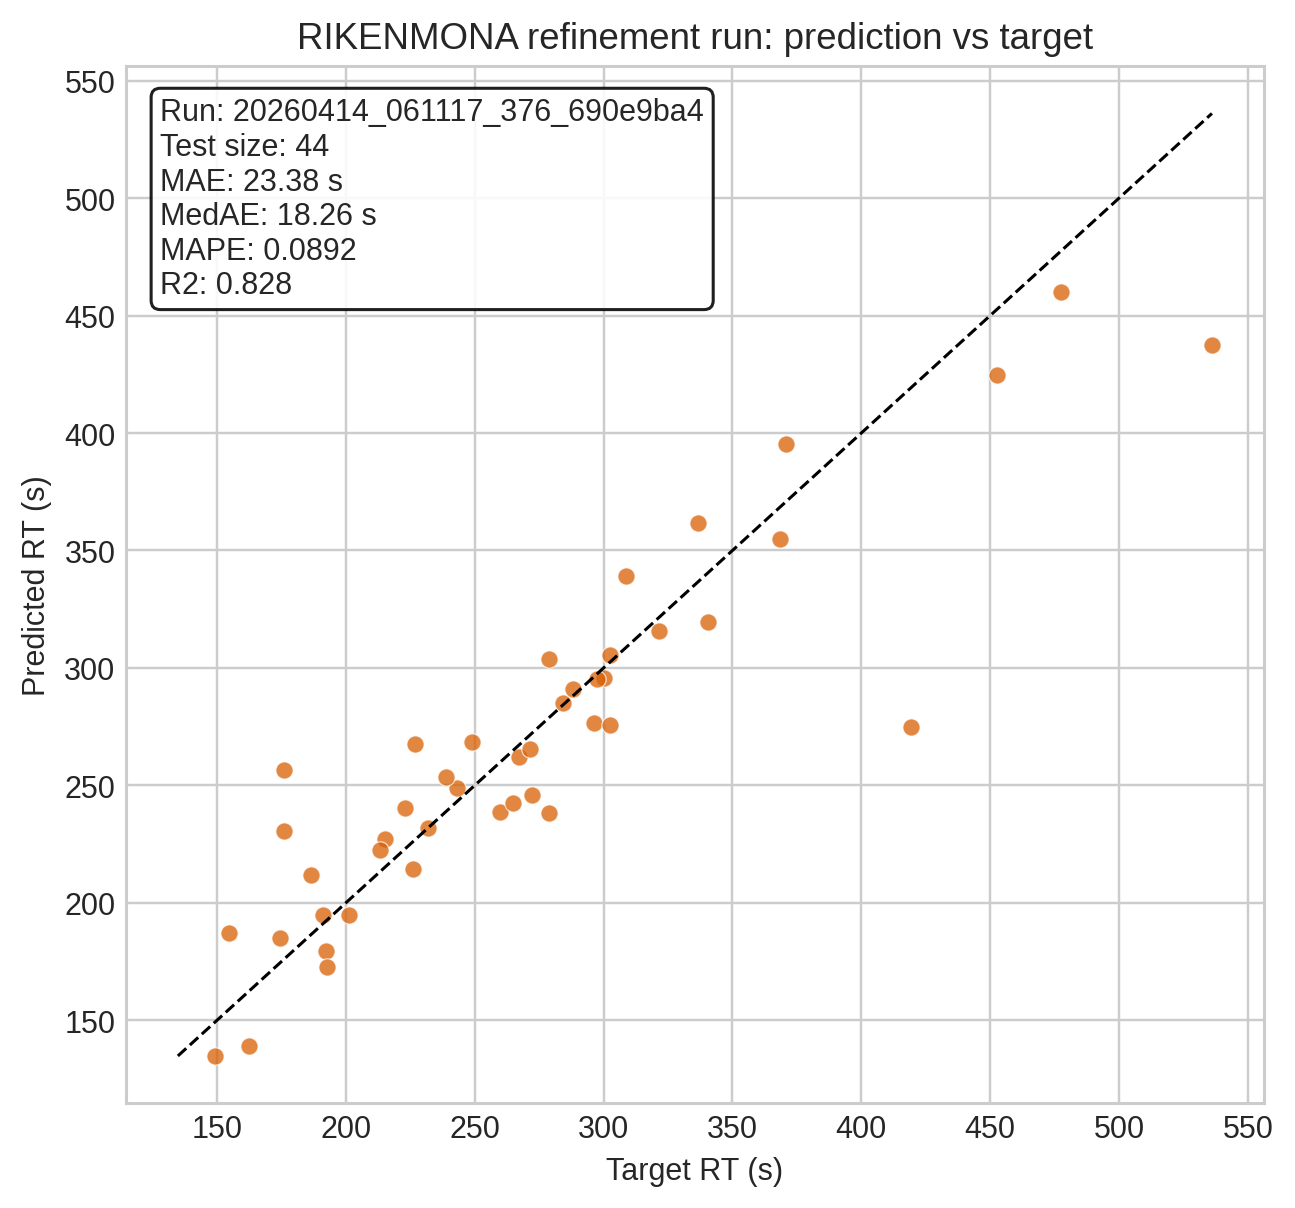
\includegraphics[width=0.68\textwidth]{Figures/riken_refined_scatter_report.png}
}{
    \fbox{\parbox{0.8\textwidth}{Run \texttt{Report/Figures/Figures.ipynb} to generate \texttt{riken\_refined\_scatter\_report.png}.}}
}
\caption{Prediction scatter plot for the RIKENMONA refinement run. This experiment is reported separately from the paper-style direct MiniDataset transfer benchmark.}
\label{fig:riken-scatter}
\end{figure}

\begin{figure}[t]
\centering
\IfFileExists{Figures/riken_mae_context_report.png}{
    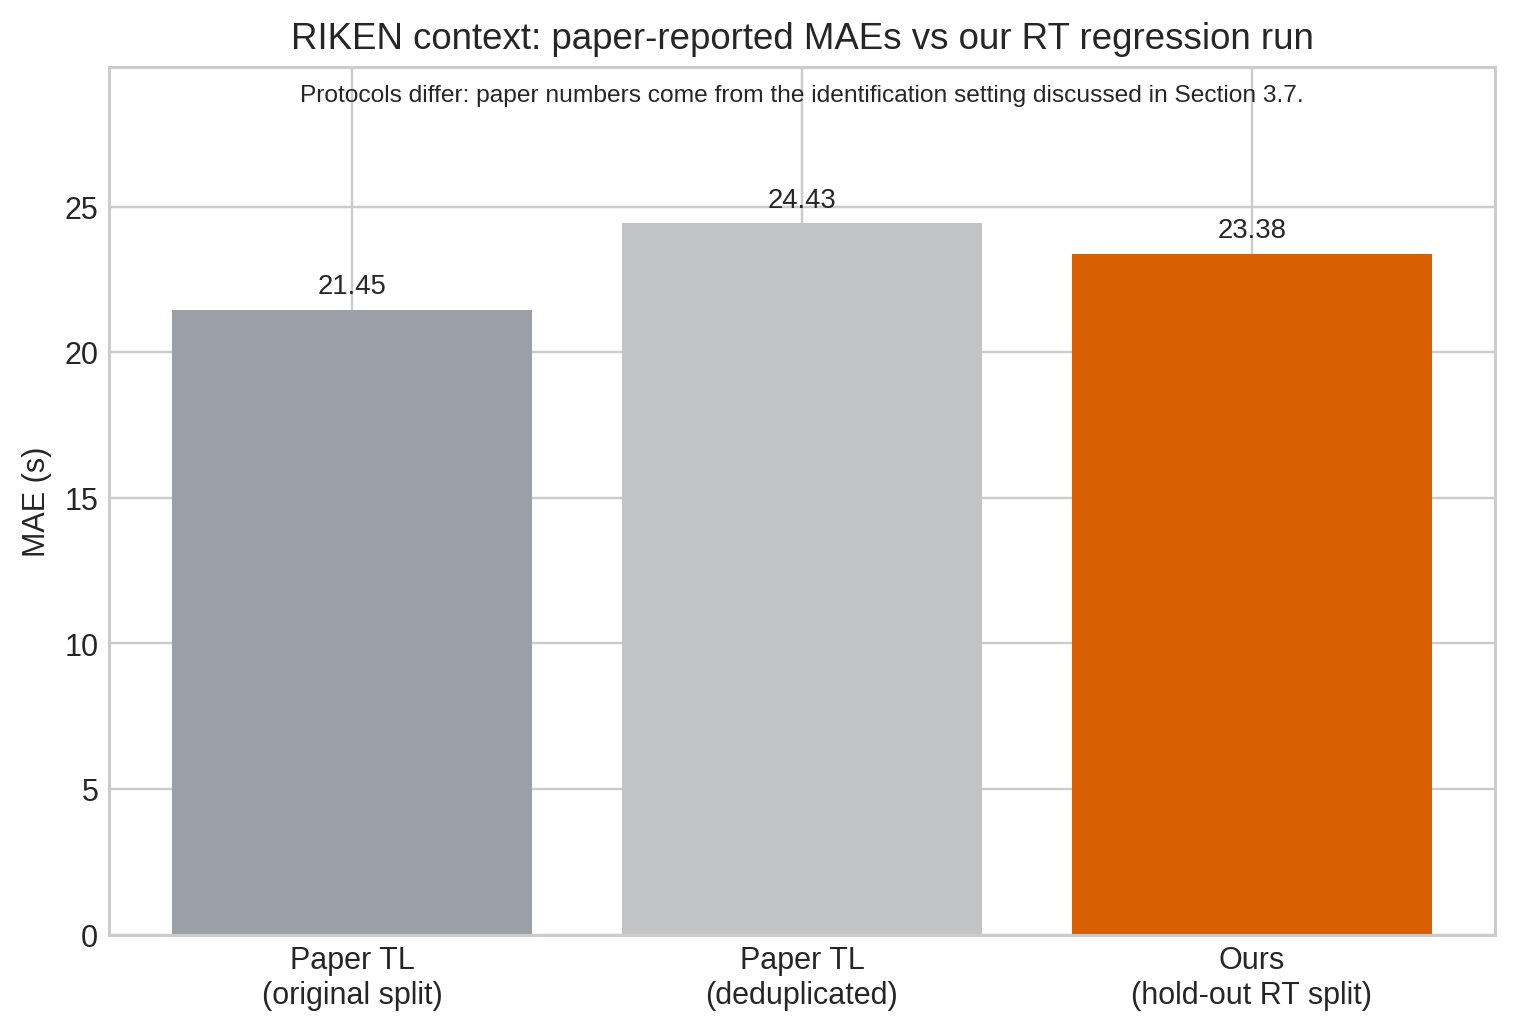
\includegraphics[width=0.72\textwidth]{Figures/riken_mae_context_report.png}
}{
    \fbox{\parbox{0.8\textwidth}{Run \texttt{Report/Figures/Figures.ipynb} to generate \texttt{riken\_mae\_context\_report.png}.}}
}
\caption{RIKEN MAE context. The paper reports \(21.45\) s on the original RIKEN-PlaSMA split and \(24.43\) s after de-duplication, while our RT-regression refinement run gives \(23.38\) s. These values are informative, but they are not strictly protocol-matched.}
\label{fig:riken-mae}
\end{figure}

The paper states that DeepGCN-RT-TL reaches a test MAE of \textbf{21.45 s} on the original RIKEN-PlaSMA split and \textbf{24.43 s} after de-duplication. Our \textbf{23.38 s} value falls between those two reference points. This is encouraging, but the comparison remains approximate because the official RIKEN numbers are tied to the identification setting described in Section 3.7, not to our current hold-out RT-regression run.

\subsection{MiniDataset Transfer Learning on the Seven Paper Datasets}

Table~\ref{tab:transfer-seven} compares the official DeepGCN-RT transfer-learning summary against our current \textbf{direct SMRT-initialized 10-fold runs} on the seven datasets discussed in the paper. To match the official result-table logic, our reported number for each dataset is the \textbf{simple average of the fold-level test MAEs recorded in \path{summary.csv}}. On these seven common datasets, the official mean MAE is \textbf{47.54 s}, while our current \textbf{1 seed \(\times\) 10 folds} mean MAE is \textbf{70.48 s}.

\begin{table}[t]
\centering
\caption{Transfer-learning MAE comparison on the seven datasets explicitly discussed in the paper. Official numbers are taken from Table 4 / \texttt{result\_summary.xlsx}. Our numbers are the mean and standard deviation over the 10 fold rows in each dataset's \texttt{summary.csv}.}
\label{tab:transfer-seven}
\begin{tabular}{lrrrr}
\toprule
Dataset & Official MAE (s) & Our mean MAE (s) & Our fold std (s) & Gap (s) \\
\midrule
Eawag\_XBridgeC18\_364 & 45.97 & 58.43 & 8.87 & +12.46 \\
FEM\_lipids\_72 & 74.48 & 107.71 & 64.21 & +33.23 \\
FEM\_long\_412 & 110.89 & 145.37 & 48.24 & +34.48 \\
IPB\_Halle\_82 & 21.20 & 59.11 & 12.52 & +37.91 \\
LIFE\_new\_184 & 18.13 & 28.22 & 7.75 & +10.09 \\
LIFE\_old\_194 & 12.07 & 21.60 & 7.86 & +9.53 \\
UniToyama\_Atlantis\_143 & 50.03 & 72.93 & 26.47 & +22.89 \\
\bottomrule
\end{tabular}
\end{table}

The overall trend is now much clearer than under the earlier one-split evaluation: our results are still worse than the official ones on all seven paper datasets, but the gaps are now measured under a more comparable aggregation rule. The smallest gap is on \texttt{LIFE\_new\_184} (\(+10.09\) s), while the largest among the seven paper datasets is on \texttt{IPB\_Halle\_82} (\(+37.91\) s). Because the paper averages over \textbf{100} fold-level results per dataset (10 seeds \(\times\) 10 folds), while we currently average over only \textbf{10} fold-level results, some residual mismatch is still expected.

\begin{figure}[t]
\centering
\IfFileExists{Figures/mini_all_mae_comparison_cv.png}{
    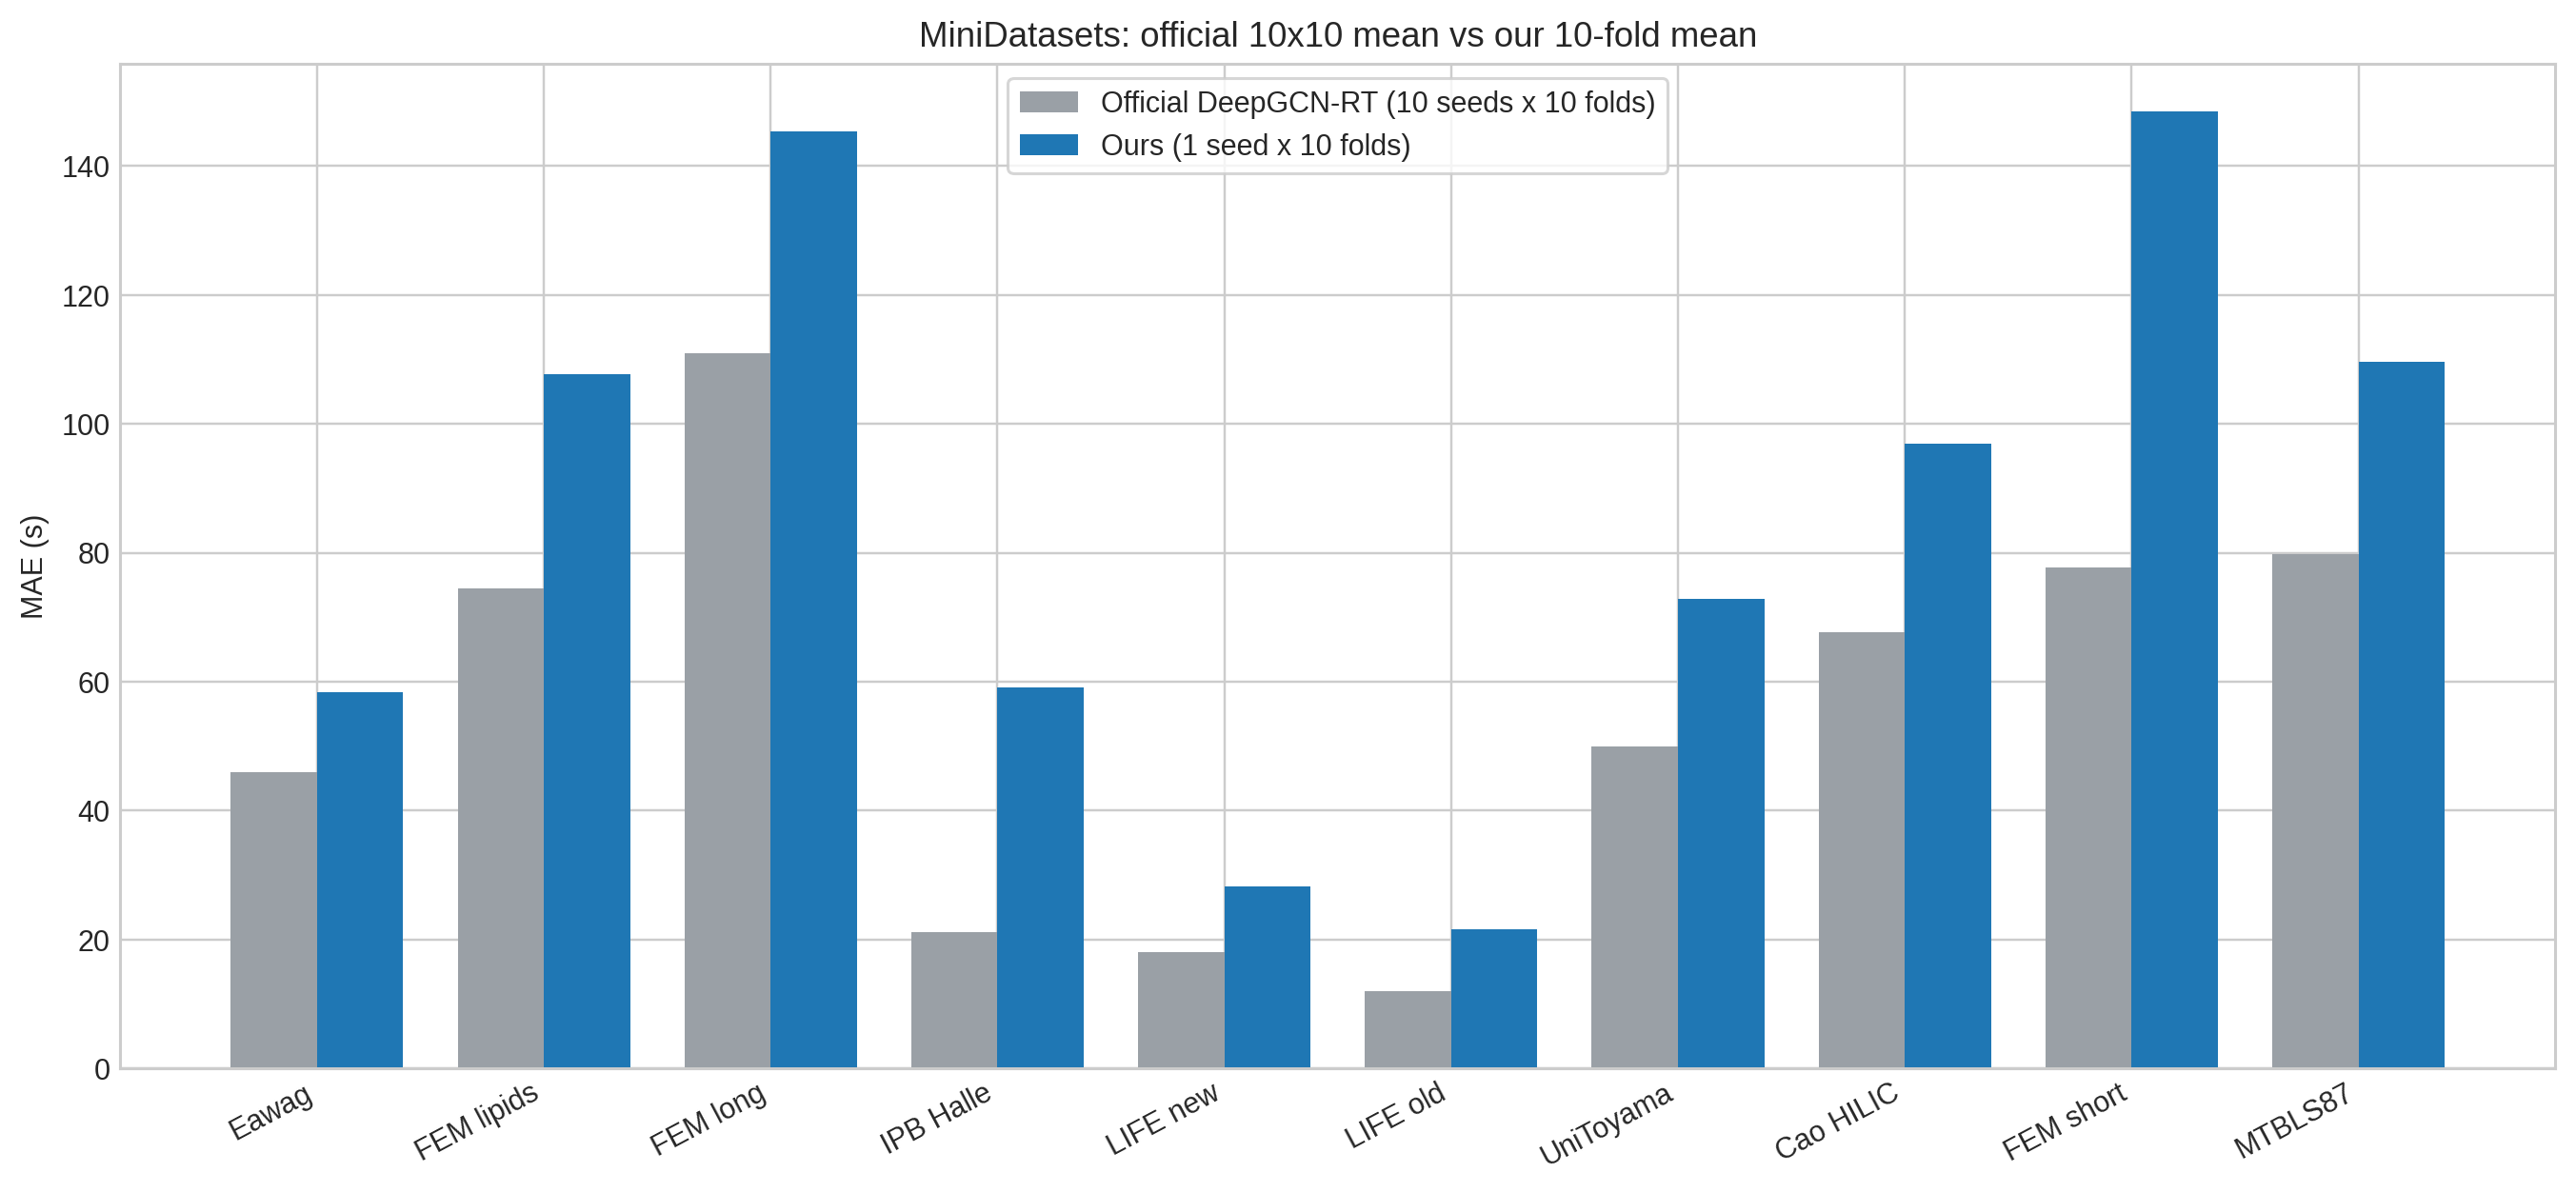
\includegraphics[width=\textwidth]{Figures/mini_all_mae_comparison_cv.png}
}{
    \fbox{\parbox{0.85\textwidth}{Run \texttt{Report/Figures/Figures.ipynb} to generate \texttt{mini\_all\_mae\_comparison\_cv.png}.}}
}
\caption{MAE comparison between the official DeepGCN-RT transfer-learning summary and our current 10-fold MiniDataset runs. The official bars summarize 10 seeds \(\times\) 10 folds; our bars summarize 1 seed \(\times\) 10 folds.}
\label{fig:mini-all-mae}
\end{figure}

\subsection{Additional Datasets Present in the Official Code}

The authors' released repository also reports three extra datasets that are not part of the main seven-dataset paper table. We ran them as well because they are already included in our data pipeline.

\begin{table}[t]
\centering
\caption{Supplementary comparison on extra datasets included in the released codebase. Official numbers come from \texttt{result\_summary.xlsx}; our numbers are 10-fold means from \texttt{summary.csv}.}
\label{tab:transfer-extra}
\begin{tabular}{lrrrr}
\toprule
Dataset & Official MAE (s) & Our mean MAE (s) & Our fold std (s) & Gap (s) \\
\midrule
Cao\_HILIC\_116 & 67.64 & 96.98 & 25.80 & +29.34 \\
FEM\_short\_73 & 77.70 & 148.44 & 50.28 & +70.74 \\
MTBLS87\_147 & 79.74 & 109.60 & 30.11 & +29.87 \\
\bottomrule
\end{tabular}
\end{table}

Across all ten transfer datasets contained in the official code, the official mean MAE is \textbf{55.79 s}, whereas our current mean MAE is \textbf{84.84 s}. The extra datasets remain difficult, especially \texttt{FEM\_short\_73}, but the gap is now substantially smaller than in the earlier single-split analysis because we no longer report one particularly lucky or unlucky fold as the final number.

\begin{figure}[t]
\centering
\IfFileExists{Figures/mini_mae_gap_sorted_cv.png}{
    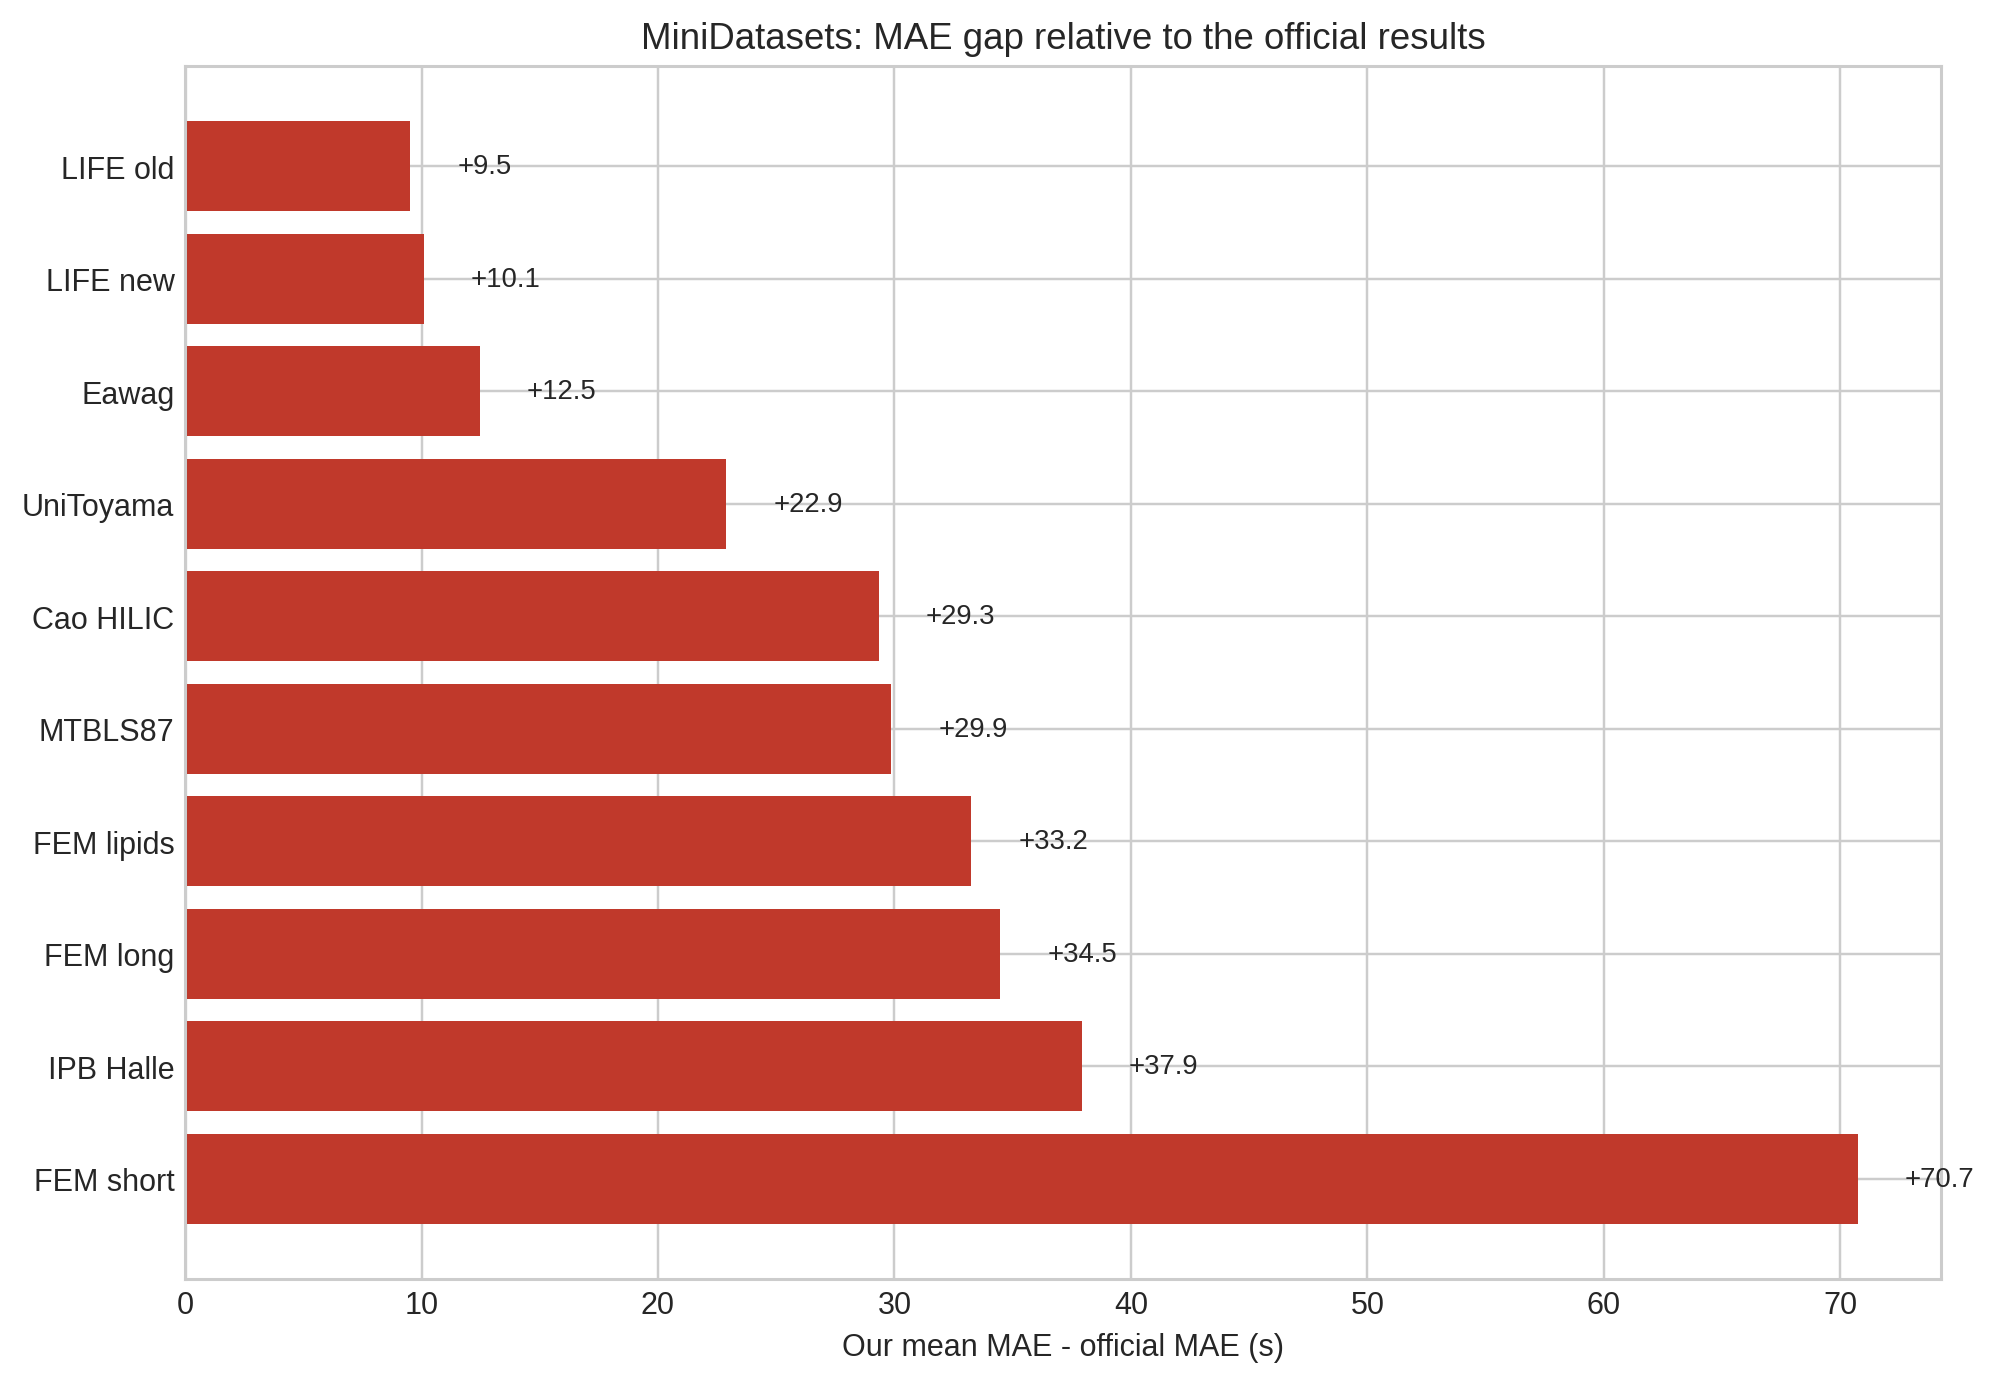
\includegraphics[width=0.86\textwidth]{Figures/mini_mae_gap_sorted_cv.png}
}{
    \fbox{\parbox{0.85\textwidth}{Run \texttt{Report/Figures/Figures.ipynb} to generate \texttt{mini\_mae\_gap\_sorted\_cv.png}.}}
}
\caption{MAE gap between our MiniDataset 10-fold means and the official DeepGCN-RT values. Positive values indicate that our MAE is larger.}
\label{fig:mini-gap}
\end{figure}

\begin{figure}[t]
\centering
\IfFileExists{Figures/mini_test_size_vs_gap_cv.png}{
    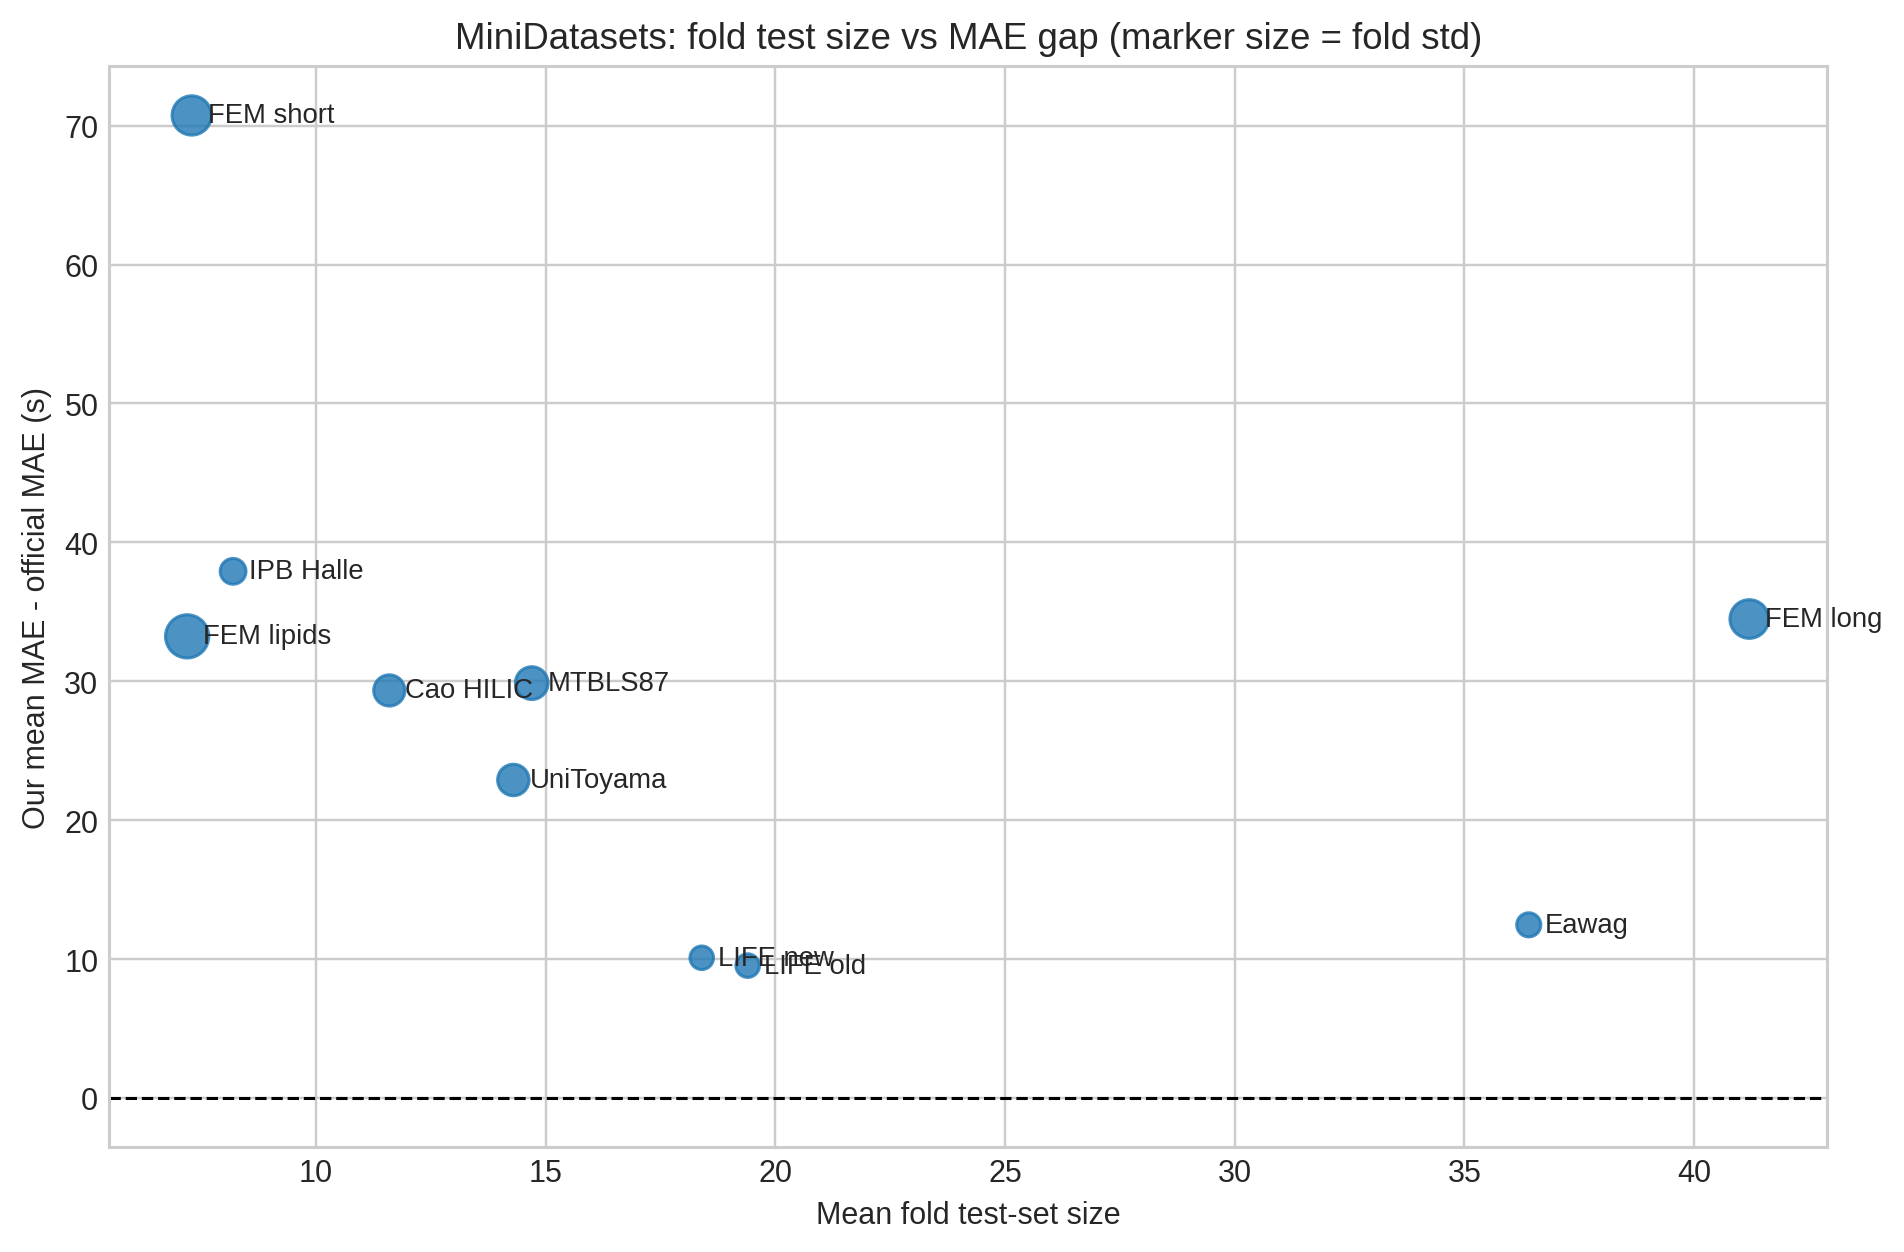
\includegraphics[width=0.78\textwidth]{Figures/mini_test_size_vs_gap_cv.png}
}{
    \fbox{\parbox{0.85\textwidth}{Run \texttt{Report/Figures/Figures.ipynb} to generate \texttt{mini\_test\_size\_vs\_gap\_cv.png}.}}
}
\caption{Relationship between mean fold test-set size and the MAE gap relative to the official results. Marker size is proportional to the standard deviation across our folds, which helps show how small datasets remain the most unstable even after switching to 10-fold evaluation.}
\label{fig:mini-testsize-gap}
\end{figure}

\section{Analysis and Discussion}

\subsection{Why Do Some Results Match Well While Others Do Not?}

The most important observation is that \textbf{SMRT matches well, the separate RIKENMONA refinement run is reasonable, but MiniDataset transfer remains weaker than the official summary even after switching to 10-fold aggregation}. This pattern strongly suggests that the \emph{model architecture} was reproduced successfully, while the remaining discrepancy is dominated by \emph{protocol differences and small-data variance} rather than by a catastrophic implementation bug.

There are five reasons for this:

\begin{enumerate}
    \item \textbf{Different SMRT split.} Our SMRT test score is close to the paper, but the split changed. A close score under a different split supports the correctness of the reimplementation, yet it is not a formal reproduction of the exact benchmark.
    \item \textbf{We only match the fold-wise aggregation, not the full 10\(\times\)10 protocol.} The paper averages over 10 seeds \(\times\) 10 folds, whereas we currently average over one seed \(\times\) 10 folds. This already reduces variance substantially compared with a single split, but it is still not the full official repetition strategy.
    \item \textbf{Checkpoint selection is stricter in our code.} The official transfer script chooses the best model by monitoring the held-out fold itself, while our implementation keeps a separate validation partition inside the training portion of each fold. This is methodologically cleaner, but it should also be expected to yield less optimistic test-fold MAEs.
    \item \textbf{Tiny test folds still amplify variance.} Several transfer datasets still have mean fold test sizes of only \textbf{7--15} molecules. Figures~\ref{fig:mini-gap} and \ref{fig:mini-testsize-gap} show that the smallest datasets remain both the noisiest and the furthest from the official summary.
    \item \textbf{Batch size and optimization settings differ in transfer learning.} The paper fine-tunes with batch size 8, whereas our current runs used batch size 64. On tiny datasets this materially changes the optimization dynamics.
\end{enumerate}

\subsection{Sensitivity to Hyperparameters and Randomness}

Even with 10-fold averaging, the logs already show clear sensitivity. The standard deviation of fold-level MAE is \textbf{64.21 s} on \texttt{FEM\_lipids\_72}, \textbf{50.28 s} on \texttt{FEM\_short\_73}, and \textbf{48.24 s} on \texttt{FEM\_long\_412}. By contrast, the more stable \texttt{LIFE\_new\_184} run still shows a fold-level MAE standard deviation of \textbf{7.75 s}. The best checkpoint epoch also varies widely within a dataset: for example, \texttt{UniToyama\_Atlantis\_143} selects epochs between \textbf{6} and \textbf{83} across folds, while \texttt{LIFE\_old\_194} ranges from \textbf{32} to \textbf{137}. This is direct evidence that small-dataset transfer learning remains highly sensitive to the exact fold composition and validation noise.

The same conclusion is visible in the mean metrics. For example, \texttt{LIFE\_new\_184} reaches a relatively low mean MAE of \(28.22\) s, but \texttt{LIFE\_old\_194} still has a much lower mean \(R^2\) (\(0.471\)) than one might expect from its MAE. By contrast, \texttt{FEM\_long\_412} has a much larger mean MAE, \(145.37\) s, but a high mean \(R^2\) of \(0.918\), meaning that the ranking structure of RT values is captured better than the absolute scale.

\subsection{Strengths and Weaknesses of the Architecture}

The project still supports the core claims of the paper:

\begin{enumerate}
    \item \textbf{Depth is useful when residual connections are present.} The 16-layer model trains stably on SMRT and reaches near-paper performance.
    \item \textbf{Edge information is valuable.} The model's best configuration is the edge-aware version, consistent with the paper's ablation conclusions.
    \item \textbf{The attentive readout is reasonable for molecular RT prediction.} The attention/GRU readout provides a natural way to summarize graph-wide interactions after deep message passing.
    \item \textbf{The RIKENMONA refinement stage is meaningful.} Its own MAE of \(23.38\) s indicates that the intermediate experiment is not arbitrary; it learns a usable RT representation on a much smaller dataset.
\end{enumerate}

At the same time, our experiments also highlight the weaknesses of the architecture in practice:

\begin{enumerate}
    \item \textbf{Transfer results are fragile on very small datasets.} Deep models can overfit quickly when there are fewer than 100 molecules.
    \item \textbf{Reported gains depend strongly on the evaluation protocol.} Averaged cross-validation and a single random split can tell very different stories.
    \item \textbf{Strict validation lowers optimism.} Keeping a separate validation partition inside each fold is methodologically cleaner, but it tends to expose the true difficulty of the smallest datasets.
    \item \textbf{The full real-world pipeline is larger than RT regression alone.} The paper's identification result depends on downstream candidate filtering, which is not reproduced by the current codebase.
\end{enumerate}

\subsection{What We Learned from the Reimplementation}

The main technical lesson is that \textbf{architectural reproduction and experimental reproduction are different tasks}. We successfully rebuilt the model family and recovered the main SMRT behavior, and we now match the paper's transfer-learning aggregation rule at the fold level, but we still do not reproduce the exact SMRT split, the official multi-seed repetition strategy, or the optimistic checkpoint-selection rule used in the released transfer script.

The second lesson is that \textbf{small changes in protocol matter a lot} on small chromatographic datasets. Merging the official SMRT train/test files, using one seed instead of ten, selecting checkpoints with a clean validation split instead of the held-out fold, and changing the transfer-learning batch size are enough to create large performance gaps even when the network architecture is essentially correct.

\section{Conclusion and Lessons Learned}

This project produced an independent PyTorch Geometric reimplementation of DeepGCN-RT and verified that the core model architecture is sound. On SMRT, our implementation achieved \textbf{26.65 s} test MAE, which is extremely close to the paper's \textbf{26.55 s}. This is the strongest evidence that the message-passing layers, residual design, readout module, and regression head were reproduced correctly. The separate RIKENMONA refinement run also behaved reasonably, reaching \textbf{23.38 s} MAE on its own hold-out split, which lies between the paper's reported original and de-duplicated RIKEN MAEs.

The downstream MiniDataset results remain weaker than the official results, but the discrepancy is now easier to interpret because the reported score is a 10-fold mean rather than a single split. On the seven common paper datasets, our mean MAE is \textbf{70.48 s} versus the official \textbf{47.54 s}; across all ten datasets in the released code, our mean MAE is \textbf{84.84 s} versus the official \textbf{55.79 s}. The remaining gap is explainable: the exact SMRT split was not preserved, the transfer-learning batch size is still 64 instead of 8, we average over one seed instead of ten, and our checkpoint-selection rule is stricter than the official transfer script. Therefore, the current report should be read as a \textbf{successful architectural reimplementation with a substantially better-aligned, but still not fully matched, experimental reproduction}.

The most direct next step would be to align the protocol exactly with the paper: preserve the official SMRT test split, rerun transfer learning with \textbf{10 seeds \(\times\) 10 folds} and batch size 8, optionally reproduce the official held-out-fold checkpoint selection for a like-for-like comparison, and implement the RIKEN candidate-filtering workflow. That would turn this project from a strong reimplementation into a much tighter numerical reproduction.

\begin{thebibliography}{9}

\bibitem{kang2023deepgcnrt}
Q. Kang, P. Fang, S. Zhang, H. Qiu, and Z. Lan,
\newblock ``Deep graph convolutional network for small-molecule retention time prediction,''
\newblock \emph{Journal of Chromatography A}, vol. 1711, 464439, 2023.

\bibitem{deepgcnrtcode}
Q. Kang et al.,
\newblock ``DeepGCN-RT official source code and pretrained models,''
\newblock GitHub repository: \url{https://github.com/kangqiyue/DeepGCN-RT}.

\end{thebibliography}
